\section{\dbsp expressivity}\label{sec:expressivity}

\subsection{Formal verification}

We have formalized and verified all the definitions, lemmas,
propositions, theorems, and examples in this paper using the Lean
theorem prover; we make these proofs available at~\cite{dbsp-theory}.
The formalization builds on mathlib~\cite{mathlib2020}, which provides
support for groups and functions with finite support (modeling
\zrs). We believe the simplicity of \dbsp enabled completing these
proofs in relatively few lines of Lean code (5K) and keeping a close
correspondence between the paper proofs in~\cite{tr} and Lean.  The
existence of the proofs bolsters our confidence in the correctness of
our implementation.

\vspace{-3ex}
\subsection{Beyond relational queries}\label{sec-turing}

\dbsp can express programs that go beyond Datalog, SQL, or incremental
versions of these: see the non-monotonic semantics for Datalog$^\neg$
and Datalog$^{\neg\neg}$\cite{Abiteboul-book95}.  \dbsp can model many
classes of streaming operators and stateful streaming computations.

For example, to illustrate the Turing-completeness of \dbsp, we
implement the following \emph{while} program, where $Q$ is an
arbitrary query: {\small
\begin{lstlisting}[language=Pascal]
x := i;
while (x changes)
    x := Q(x);
\end{lstlisting}}
The \dbsp implementation of this program is:

%$$\lambda i. \int[\D[\fix{\xi}{Q(\delta(i)+\zm(\xi))}]]$$
\begin{center}
\begin{tikzpicture}[>=latex]
  \node[] (input) {$i$};
  \node[block, right of=input] (delta) {$\delta$};
  \node[block, circle, right of=delta, inner sep=0cm] (p) {$+$};
  \node[block, right of=p] (Q) {$\lift Q$};
  \node[block, right of=Q] (D) {$\D$};
  \node[block, right of=D] (S) {$\int$};
  \node[right of=S] (output)  {$x$};
  \node[block, below of=p, node distance=.8cm] (z) {$\zm$};
  \draw[->] (input) -- (delta);
  \draw[->>] (delta) -- (p);
  \draw[->>] (p) -- (Q);
  \draw[->>] (Q) -- node (mid) {} (D);
  \draw[->>] (D) -- (S);
  \draw[->>] (mid.center) |- (z);
  \draw[->] (S) -- (output);
  \draw[->>] (z) -- (p);
\end{tikzpicture}
\end{center}

This circuit can be converted to a streaming circuit that computes a stream of values $i$
by lifting it; it can be incrementalized using Algorithm~\ref{algorithm-inc} to compute on changes of $i$:

\noindent
\begin{center}
\begin{tikzpicture}[>=latex]
  \node[] (input) {$\Delta i$};
  \node[block, right of=input] (delta) {$\lift{\delta}$};
  \node[block, circle, right of=delta, inner sep=0cm] (p) {$+$};
  \node[block, right of=p, node distance=1.3cm] (Q) {$\inc{(\lift{\lift{Q}})}$};
  \node[block, right of=Q, node distance=1.5cm] (D) {$\lift{\D}$};
  \node[block, right of=D, node distance=1.1cm] (S) {$\lift{\int}$};
  \node[right of=S, node distance=1.2cm] (output)  {$\Delta x$};
  \node[block, below of=p, node distance=.9cm] (z) {$\lift{\zm}$};
  \draw[->>] (input) -- (delta);
  \draw[->>>] (delta) -- (p);
  \draw[->>>] (p) -- (Q);
  \draw[->>>] (Q) -- node (mid) {} (D);
  \draw[->>>] (D) -- (S);
  \draw[->>>] (mid.center) |- (z);
  \draw[->>] (S) -- (output);
  \draw[->>>] (z) -- (p);
\end{tikzpicture}
\end{center}

At runtime the execution of this circuit is not guaranteed to terminate;
however, if the circuit does terminate, it will produce the correct
output, i.e., the least fixpoint of $Q$ that includes~$i$.

\subsection{Supporting SQL}\label{sec:sql}

In \secref{sec:relational} we have shown how to implement the
relational algebra using \dbsp.  However, the SQL language is
significantly richer than the relational algebra.

\paragraph{Multisets.} SQL operates on \emph{multisets} (or bags), e.g.,
\code{UNION ALL}.  Since \zrs generalize bags, they can model all SQL
operations. Many queries on multisets can be implemented by just
omitting $\distinct$ operators.

\paragraph{NULLs.} \dbsp says nothing about the data types
and the functions that are executed by the operators in each node.  In
our Rust SQL runtime (described in Section~\refsec{sec:runtime})
nullable types are represented using Rust \texttt{Option<>} types, and
SQL \code{NULL} is the value \code{None}.  Some care is required in
implementing the unusual semantics of \code{NULL} (e.g., in SQL two
\code{NULL} values are neither equal, nor different).

\paragraph{Primary keys.} A primary key changes a table's behavior on insertion:
inserting a tuple can cause another tuple to be deleted.  This
behavior looks roughly like a modified $\distinct$ operator, and can
be implemented incrementally similarly:

\begin{center}
\begin{tikzpicture}[>=latex]
    \node[] (input) {$\Delta d$};
    \node[block, right of=input] (I) {$\I$};
    \node[block, right of=I] (z) {$\zm$};
    \node[block, below of=z, node distance=.8cm] (H) {\texttt{UPSERT}};
    \node[right of=H, node distance=1.3cm] (output) {$\Delta o$};
    \draw[->>] (input) -- node (mid) {} (I);
    \draw[->>] (I) -- (z);
    \draw[->>] (mid.center) |- (H);
    \draw[->>] (z) -- node (i) [right] {} (H);
    \draw[->>] (H) -- (output);
\end{tikzpicture}
\end{center}

\noindent The \code{UPSERT} operator converts a \zr describing an
insertion with key $k$: $\{ (k, v) \mapsto 1 \}$ to a \zr $\{ (k, v)
\mapsto 1, (k, v') \mapsto -1 \}$, where $(k, v')$ is the previous
value of the record, obtained from the $\I$ operator.

\paragraph{Constant values.}  One can write in SQL queries that have
constant outputs, e.g., \code{SELECT 2}.  Technically an operator that
produces a constant result is not TI.  However, constants can be
accommodated easily by modeling them mathematically as constant input
streams.

\subsubsection{Grouping and indexed \zrs}\label{sec:grouping}

Let $K$ be a set of ``key'' values.  The finite maps from $K$ to \zrs
are functions $K \to \Z[A] = \Z[A][K]$.  We call values $i$ of this
type \defined{indexed \zrs}: for each key $k \in K$, $i[k]$ is a \zr.
Because the codomain $\Z[A]$ is an Abelian group, this structure is
itself an Abelian group.  Here is an example indexed \zr:

\begin{center}
  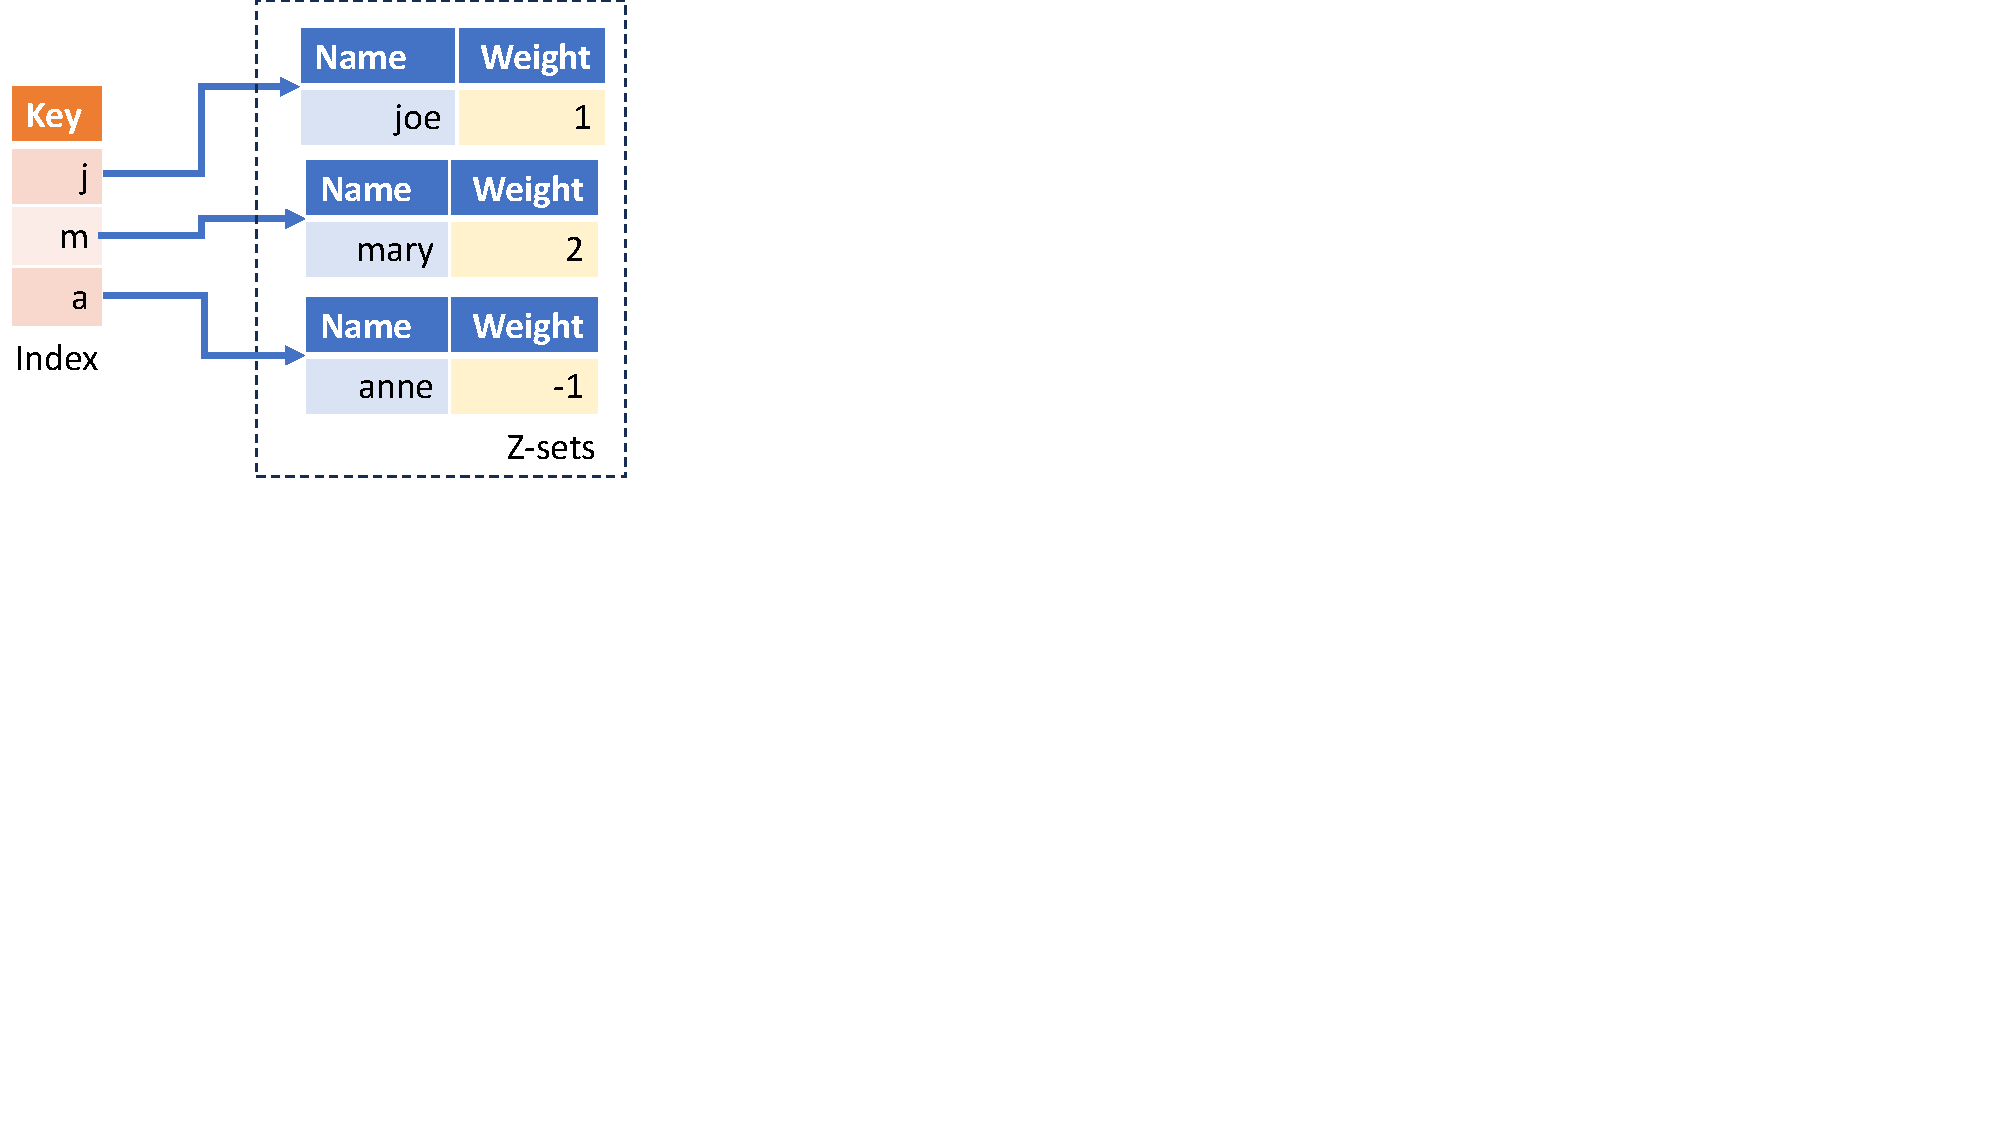
\includegraphics[trim={0 4.2in 7.5in 0},clip,scale=.34]{indexed.pdf}
\end{center}

This structure is used to implement the SQL \texttt{GROUP BY} operator
in \dbsp.  Consider a \defined{partitioning function} $p: A \to K$
that assigns a key to any value in $A$.  We define the grouping
function $G_p: \Z[A] \to \Z[A][K]$ as $G_p(a)[k] \defn \sum_{x \in
  a.p(x)=k}\{ x \mapsto a[x] \}$ (just map each element of the input
$a$ to the \zr grouping corresponding to its key).  When applied to a
\zr this function returns an indexed \zr: each key $k$ maps to a \zr
containing all elements of the group (as in SQL, each group is a
multiset).  Consider our example \zr $R$ from \refsec{sec:relational},
and a key function $p(s)$ that returns the first letter of the string
$s$.  The resulting indexed \zr is shown in the previous diagram.

The operation building an indexed \zr from a \zr is linear for any key
function!  It follows that group-by is incremental: each row changed
in the input relation produces a row changed in a group, obtained by
applying the partitioning function.

Notice that, unlike SQL, \dbsp can express naturally computations on
indexed \zrs, they are just an instance of a group structure.  In
\dbsp one does not need to follow grouping by aggregation, and \dbsp
can represent nested groupings of arbitrary depth.  Indeed, our
compiler can recognize classes of such computations expressed using
SQL windows (e.g., TopK for each group), and can generate efficient
incremental code.

%Please note that our definition of incremental computation is only
%concerned with incrementality in the \emph{outermost} structures.  We
%leave it to future work to explore an appropriate definition of
%incremental computation on the \emph{inner} relations.

%\subsubsection{\texttt{UNNEST} (flatmap)}

A useful operation on indexed \zrs is \defined{flatmap} (or
\code{UNNEST} in SQL), which one can view as the inverse of grouping,
converting an indexed \zr into a \zr.  This operation is also a linear
\dbsp operator.

\subsubsection{Aggregation}\label{sec:aggregation}

Aggregation in SQL applies a function $a$ to a set of values of type
$A$ producing a ``scalar'' result with some result type $B$.  In \dbsp
an aggregation function has a signature $a: \Z[A] \to B$.  When
operating on \zrs, most aggregation functions have to multiply the
contribution of each value by its associated weight (but not
aggregates such as \code{MAX}).  \texttt{DISTINCT} aggregates have to
first apply a \texttt{DISTINCT} operator.

Distributive (e.g. \code{SUM}) and some algebraic aggregation
(\code{AVG}) functions can be implemented by a pair of linear
functions between \zrs and the target group: the actual aggregation
and the post-processing (e.g., dividing the sum by the counter for
average).  Since these are linear functions, it would seem that they
can be implemented using linear operators in \dbsp.  However, this is
not true!

The subtle point is that in SQL the result of these aggregation must
be a (singleton) \textbf{set} containing an element of $B$, and not a
value with type $B$.  Thus an aggregate based on a linear function is
decomposed into a linear \dbsp operator, followed by additional
operators, which are needed to convert the values of $B$ into values
of $\Z[B]$.  The later operators are \emph{not} linear.  Consider the
following query: \code{SELECT COUNT(*) FROM I}.  The lifted
incremental version of this query is the following circuit, where
$a_\texttt{COUNT}$ is a linear operator implementing the ``count''
aggregation function, which just sums up the weights of the input
values:

\begin{tikzpicture}[>=latex, node distance=1.2cm]
  \node[] (in) {$\Delta$\code{I}};
  \node[block, right of=in] (pi) {$\pi_\texttt{C}$};
  \node[block, right of=pi] (a) {$a_\texttt{COUNT}$};
  \node[block, right of=a] (inc) {$\mathit{inc}$};
  \node[block, below of=inc, node distance=.7cm] (IN) {$\I$};

  \node[block, right of=inc] (I) {$\I$};
  \node[block, right of=I] (z) {$\zm$};
  \node[block, below of=z, node distance=.8cm] (H) {\texttt{UPSERT}};
  \node[right of=H, node distance=1.3cm] (output) {$\Delta o$};
  \draw[->>] (in) -- (pi);
  \draw[->>] (pi) -- (a);
  \draw[->>] (a) |- (IN);
  \draw[->>] (IN) -- (inc);
  \draw[->>] (a) -- (inc);
  \draw[->>] (I) -- (z);
  \draw[->>] (z) -- (H);
  \draw[->>] (H) -- (output);
  \draw[->>] (inc) -- node (mm) {} (I);
  \draw[->>] (mm.center) |- (H);
\end{tikzpicture}

Let's say the input table \code{I} has 2 elements, and thus the
previous aggregation result was 2.  When adding a new row, the
$\mathit{inc}$ increments the previous aggregation result (obtained
from $\I$) result with the current increment, and then the
\code{UPSERT} converts the insertion of the tuple $\{3 \mapsto 1\}$
into the \zr $\{3 \mapsto 1, 2 \mapsto -1 \}$, since the output set no
longer contains the value 2.  The $\mathit{inc}$, $\I$ and $\makeset$
operators only do work proportional to the size of the change, and
they only store $O(1)$ state.

%An aggregation function such as \texttt{AVG} can be written as the composition of
%a linear function that computes a pair of values using
%\texttt{SUM} and \texttt{COUNT}, followed by a division and a call to \makeset.

%\begin{lstlisting}[language=SQL]
%SELECT AVG(c) FROM I
%\end{lstlisting}
%
%\begin{tikzpicture}[auto,>=latex]
%  \node[] (I) {\code{I}};
%  \node[block, right of=I] (pi) {$\pi_\texttt{C}$};
%  \node[block, right of=pi, node distance=1.4cm] (sc) {$(a_\texttt{SUM}, a_\texttt{COUNT})$};
%  \draw[->] (I) -- (pi);
%  \draw[->] (pi) -- (sc);
%  \node[block, right of=sc, node distance=1.8cm] (m) {$\makeset$};
%  \node[block, right of=m, node distance=1.2cm] (div) {$\sigma_/$};
%  \node[right of=div] (O) {\code{O}};
%  \draw[->] (sc) -- (m);
%  \draw[->] (m) -- (div);
%  \draw[->] (div) -- (O);
%\end{tikzpicture}

Aggregate functions, such as \code{MIN}, are \emph{not} linear in the
presence of deletions.  The incremental form of such aggregates needs
to maintain the entire input collection, using an $\I$ operator,
similar to the $\distinct$ operator.  They can be implemented
efficiently by keeping the data organized as a priority heap sorted by
the value compared.

In SQL, \code{NULL} values do not participate in aggregation, so one
needs to insert two extra operators for collections of nullable
values:
\begin{itemize}
  \item an operator that counts the number of rows aggregated (as
    described by Mumick~\cite{mumick-sigmod97}), which is used to
    detect empty groups
  \item a filtering operator (linear), which eliminates \code{NULL}s
    prior to aggregation
\end{itemize}

For many SQL aggregation functions aggregating over an empty set
should produce a \code{NULL} result.  All aggregation circuits
described so far will return an empty \zr for an empty input.  Let $z$
be the result expected for the empty input (e.g., \code{NULL}).  The
following circuit, applied after aggregation, will produce the result
expected by SQL:

\begin{center}
\begin{tikzpicture}[auto,>=latex]
  \node[] (agg) {\code{agg}};
  \node[right of=agg] (dummy) {};
  \node[block, above of=dummy, node distance=.7cm] (map) {$\code{map}(\lambda x . z)$};
  \node[block, right of=map, shape=circle, inner sep=0in, node distance=1.5cm] (minus) {$-$};
  \node[block, below of=minus, node distance=1.4cm] (zero) {$z$};
  \node[block, right of=agg, node distance=3cm, shape=circle, inner sep=0in] (plus) {$+$};
  \node[right of=plus] (out) {$out$};
  \draw[->] (agg) -- (map);
  \draw[->] (map) -- (minus);
  \draw[->] (minus) -- (plus);
  \draw[->] (zero) -- (plus);
  \draw[->] (agg) -- (plus);
  \draw[->] (plus) -- (out);
\end{tikzpicture}
\end{center}

\noindent When \code{agg} is the empty \zr, the ``map'' node produces
an empty \zr, and the final result is just $z$.  When \code{agg} is
non-empty, the top and bottom branches of the adder cancel each other,
and the result is \code{agg}.  This scheme is also implemented by
Materialize Inc.'s IVM engine.

\subsubsection{\texttt{GROUP BY-AGGREGATE}}

Grouping in SQL is always followed by aggregation.  This can be
modeled by the composition of our solutions for grouping and
aggregation described above.  In this case, the \code{UPSERT} operator
indexes data using the group key.  For linear aggregates this operator
needs to maintain state proportional to the number of groups.  For
aggregates based on non-linear functions, this maintains state
proportional to the entire input collection.

%If we use an aggregation function $a: K \times Z[A]$ that is linear in its
%second argument, then the aggregation operator $Agg_a$ is linear, and
%thus fully incremental.  As a consequence, $\mbox{flatmap}$ is linear.
%However, many practical aggregation functions for nested relations are in fact
%not linear; an example is the $count$ function above, which is not linear
%since it uses the $\makeset$ non-linear function.  Nevertheless, while
%the incremental evaluation of such functions is not fully incremental,
%it is at least partly incremental: when applying a change to groupings, the aggregation
%function only needs to be re-evaluated \emph{for groupings that have changed}.

%\subsection{Antijoin}\label{sec:antijoin}\index{antijoin}
%
%Antijoins arise in the implementation of Datalog programs with stratified negation.
%Consider the following program:
%
%\begin{lstlisting}[language=ddlog,basicstyle=\small]
%O(v, z) :- I1(v, z), not I2(v).
%\end{lstlisting}
%
%The semantics of such a rule is defined in terms of joins and set difference.
%This rule is equivalent with the following pair of rules:
%
%\begin{lstlisting}[language=ddlog,basicstyle=\small]
%C(v, z) :- I1(v, z), I2(v).
%O(v, z) :- I1(v, z), not C(v, z).
%\end{lstlisting}
%
%This transformation reduces an antijoin to a join
%followed by a set difference.  This produces the following \dbsp circuit:
%
%\begin{tikzpicture}[auto,>=latex]
%  \node[] (i1) {\code{I1}};
%  \node[below of=i1, node distance=.5cm] (i2) {\code{I2}};
%  \node[block, right of=i1, node distance=1.5cm] (join) {$\bowtie$};
%  \node[block, shape=circle, inner sep=0in, right of=join] (m) {---};
%  \node[block, above of=m, shape=circle, inner sep=0in, node distance=.6cm] (plus) {$+$};
%  \node[block, right of=plus, node distance=1cm] (distinct) {$\distinct$};
%  \node[right of=distinct, node distance=1cm] (output) {\code{O}};
%  \draw[->] (i1) -- node (tap) {} (join);
%  \draw[->] (i2) -| (join);
%  \draw[->] (join) -- (m);
%  \draw[->] (m) -- (plus);
%  \draw[->] (tap.south) |- (plus);
%  \draw[->] (plus) -- (distinct);
%  \draw[->] (distinct) -- (output);
%\end{tikzpicture}
%

\subsubsection{Other operations on SQL groups}

SQL constructs such as \code{PARTITION BY/OVER} make it possible to
write queries over groups, e.g., TOP-K.  These can be implemented in
\dbsp naturally as functions over indexed \zrs.  Moreover, many such
functions (\code{LAG}, \code{RANGE}) can be implemented using highly
efficient incremental \dbsp operators, which perform work proportional
to the size of the change.

\subsubsection{Recursive SQL queries}

SQL recursion is severely restricted by design~\cite{hirn-cidr23} and
has a strange semantics.  Instead of supporting standard SQL
recursion, in our implementation we have extended the SQL syntax to
support mutually recursive views by adding a statement to declare
recursive views prior to their use; the syntax is similar to SQL table
declarations: \code{DECLARE RECURSIVE VIEW V(col TYPE, ...)}. \\ We find
this syntax much easier to use and understand than the standard syntax
using common-table expressions.  There are essentially no restrictions
on the queries that can be used to define mutually recursive views;
such queries do not have to be monotone.  With this change, SQL
essentially includes Datalog as a sub-language.

